\graphicspath{{figures/intro/}}

\chapter{绪论}

\section{课题研究背景及意义}

2016 年 6 月 23 日,江苏盐城发生一场 EF4 级龙卷风,对盐城市阜宁县、射阳县一带造成严重影响。
据当局统计,龙卷风至少造成 99 死,846 人伤,其中近 200 人重伤。
此龙卷风造成的伤亡是几十年来最严重的\cite{wiki2016yancheng}。
这一严重龙卷风灾引起了社会对极端天气现象的关注。

龙卷风是一种伴随着高速旋转的漏斗状云柱的强风涡旋,中心附近风速可达 \SI{100}{m/s} -- \SI{200}{m/s},甚至 \SI{300}{m/s}。

美国国家海洋和大气管理局对美国历年记录的龙卷风发生次数和等级的统计如图\ref{fig:tornado-years}所示\cite{noaa2017tornado}:
美国每年平均记录到 $1,200$ 次龙卷风,2000年后龙卷风发生次数各年间波动较大,产生这一波动的原因还未有定论。
这意味着以后可能会出现某些年份龙卷风出现次数非常多、而其余年份次数较少的情况。

\begin{figure}[!htbp]
    \centering
    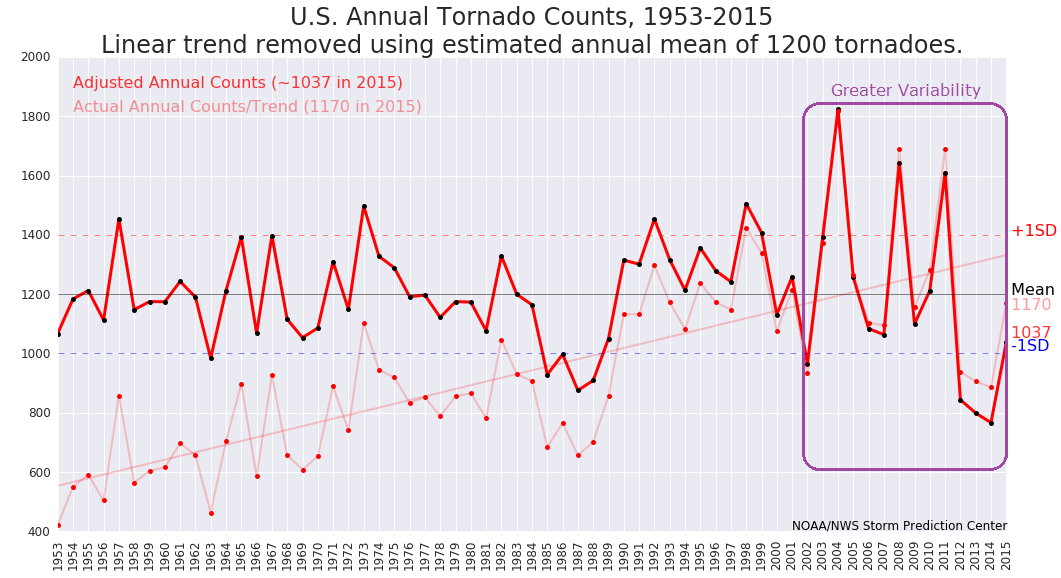
\includegraphics[width=\textwidth]{toryears.png}
    \caption{美国龙卷风年发生次数统计}
    \label{fig:tornado-years}
\end{figure}

相比于美国,中国龙卷风发生的概率相对较小,平均每年不足 100 个,大多集中在中、东部地区,如长江三角洲、苏北、鲁西南、豫东平原等。
我国龙卷风发生的数量虽然不及美国,但其造成的损失也是巨大的,据统计我国平均每年有$17$个省(区、市)遭受龙卷风,每年因龙卷风造成的死亡人数都在$10$人以上,受伤人数超千人,受灾人数更是少则上万多则百万,造成的直接经济损失高达数十亿元\cite{liu2007chinese}。

尽管龙卷风每年对我国造成的损失是巨大的,但由于其发生的概率和影响范围相对较小,目前我国《建筑结构荷载规范》中尚未包含普通建筑结构的抗龙卷风设计要求,但对一些重大工程如核电常规岛,一旦遭受破坏,其后果将不堪设想,我国已明确要求此类工程必须考虑结构的抗龙卷风设计。

大跨越输电塔结构是重要的生命线电力工程设施,具有数量大、分布广等特点,容易遭受龙卷风的袭击,其破坏将导致供电系统的瘫痪甚至引发火灾等严重后果,造成重大经济损失。

2016 年江苏盐城龙卷风中,共计 220 座各类通信基站退服,倒杆 2800 根,部分地区出现影响电力供应中断和通信基站无信号的情况,1570 根有线信号杆线受损,162 杆路灯损坏,40 条高压供电线路受损,影响 3 万负荷供电;
射阳县电力、通讯杆线受损严重,龙卷风经过的 4 条 10 千伏线路区域用户全停。
在当地的阿特斯协鑫阳光电力科技有限公司的两座厂房损毁,损毁面积达 4 万平方米\cite{thepaper2016yancheng}。
输电线路的破坏直接影响了救援救伤的效率,造成了灾区人民生命财产的重大损失。

2003 年 4 月 12 日,广东河源遭受罕见的龙卷风袭击,输电系统遭到重创,205 座高压输电线杆塔、440 条线杆被折断或者刮倒\cite{zhang2006shudianxian}。

据统计,全球范围内约$80\%$的输电塔倒塌破坏是由于极端天气(如龙卷风、雷暴等)的影响\cite{hamada2010finite}。
这主要因为大跨越输电塔结构具有塔体结构高、跨距大、柔性强等特点,是风敏感性结构,这就需要在其设计中考虑龙卷风荷载。
美国输电塔设计规范已考虑龙卷风等极端天气荷载,但我国输电线路设计规范尚未涉及。
鉴于近年龙卷风发生频率和强度似有增大趋势,而以往国内针对输电塔受龙卷风袭击的研究较少。
故为保障龙卷风多发地区电网运行安全,进行输电线路的龙卷风荷载及抗风研究具有重要的理论和实用价值。

\section{龙卷风荷载研究现状}
龙卷风是强对流天气的产物,是一种小尺度的高速旋转的气旋,具有突发性、区域性、短暂性、强破坏性,其风场特性不同于常规风。
迄今为止,人们对于龙卷风的发生机理尚未彻底清楚,但学者从未停止对龙卷风的研究。
从早期气象上的理论和实测研究,到如今的试验和数值模拟研究,获得了可供工程设计参考的相关数据。
这一过程中,龙卷风风场结构及其荷载的研究方法在不断地发展进步。
目前,国内外对龙卷风荷载的研究主要有现场实测、理论分析、试验模拟和数值模拟等方法,下文逐一介绍。

\subsection{现场实测研究}
现场实测是研究龙卷风最直直接且重要的方法。
但由于龙卷风发生地点及移动路径的随机性,研究者无法事先在其移动路径上安置观测仪器。
另外,龙卷风破坏力巨大,风场中常夹杂着飞射物,观测仪器容易遭受破坏丧失数据采集能力。
另一种现场实测方法是采用可移动的 Doppler 雷达来追踪并测量龙卷风。
但由于测量设备的限制,无法获得近地面风场的准确数据,而近地面数据又是工程抗龙卷风设计的重要参考数据,
这限制了现场实测数据在实际工程抗龙卷风设计中的应用。

即便如此,现场实测仍然为龙卷风风场结构、演化规律等的研究提供的宝贵数据。
爱荷华州立大学利用一种非常坚固的探测仪器,并在其内部设置朝向八个方向的摄像头,以便能从不同角度拍摄龙卷风内部情况。
根据拍摄的录像可以看到,龙卷风袭击低矮房屋时,房屋各个部分的破坏顺序为:首先是屋顶坍塌,然后是周围墙壁,最后是整个房屋倒塌。
房屋首先受到底部巨大风速的冲击,接着被旋风从外围袭击,最后被向上的气流摧毁。
Alexander(2005)\cite{alexander200530}利用移动的 Doppler 雷达获得了 1998 年 5 月 30 日发生于美国南达科他州的强龙卷风不同高度处的风速。
Kuai(2008)\cite{kuai2008cfd}等人对其数据进行处理,得到该龙卷风切向和径向风速分布分别如图\ref{fig:vt}和\ref{fig:vr}所示。
\begin{figure}[!htbp]
    \centering
    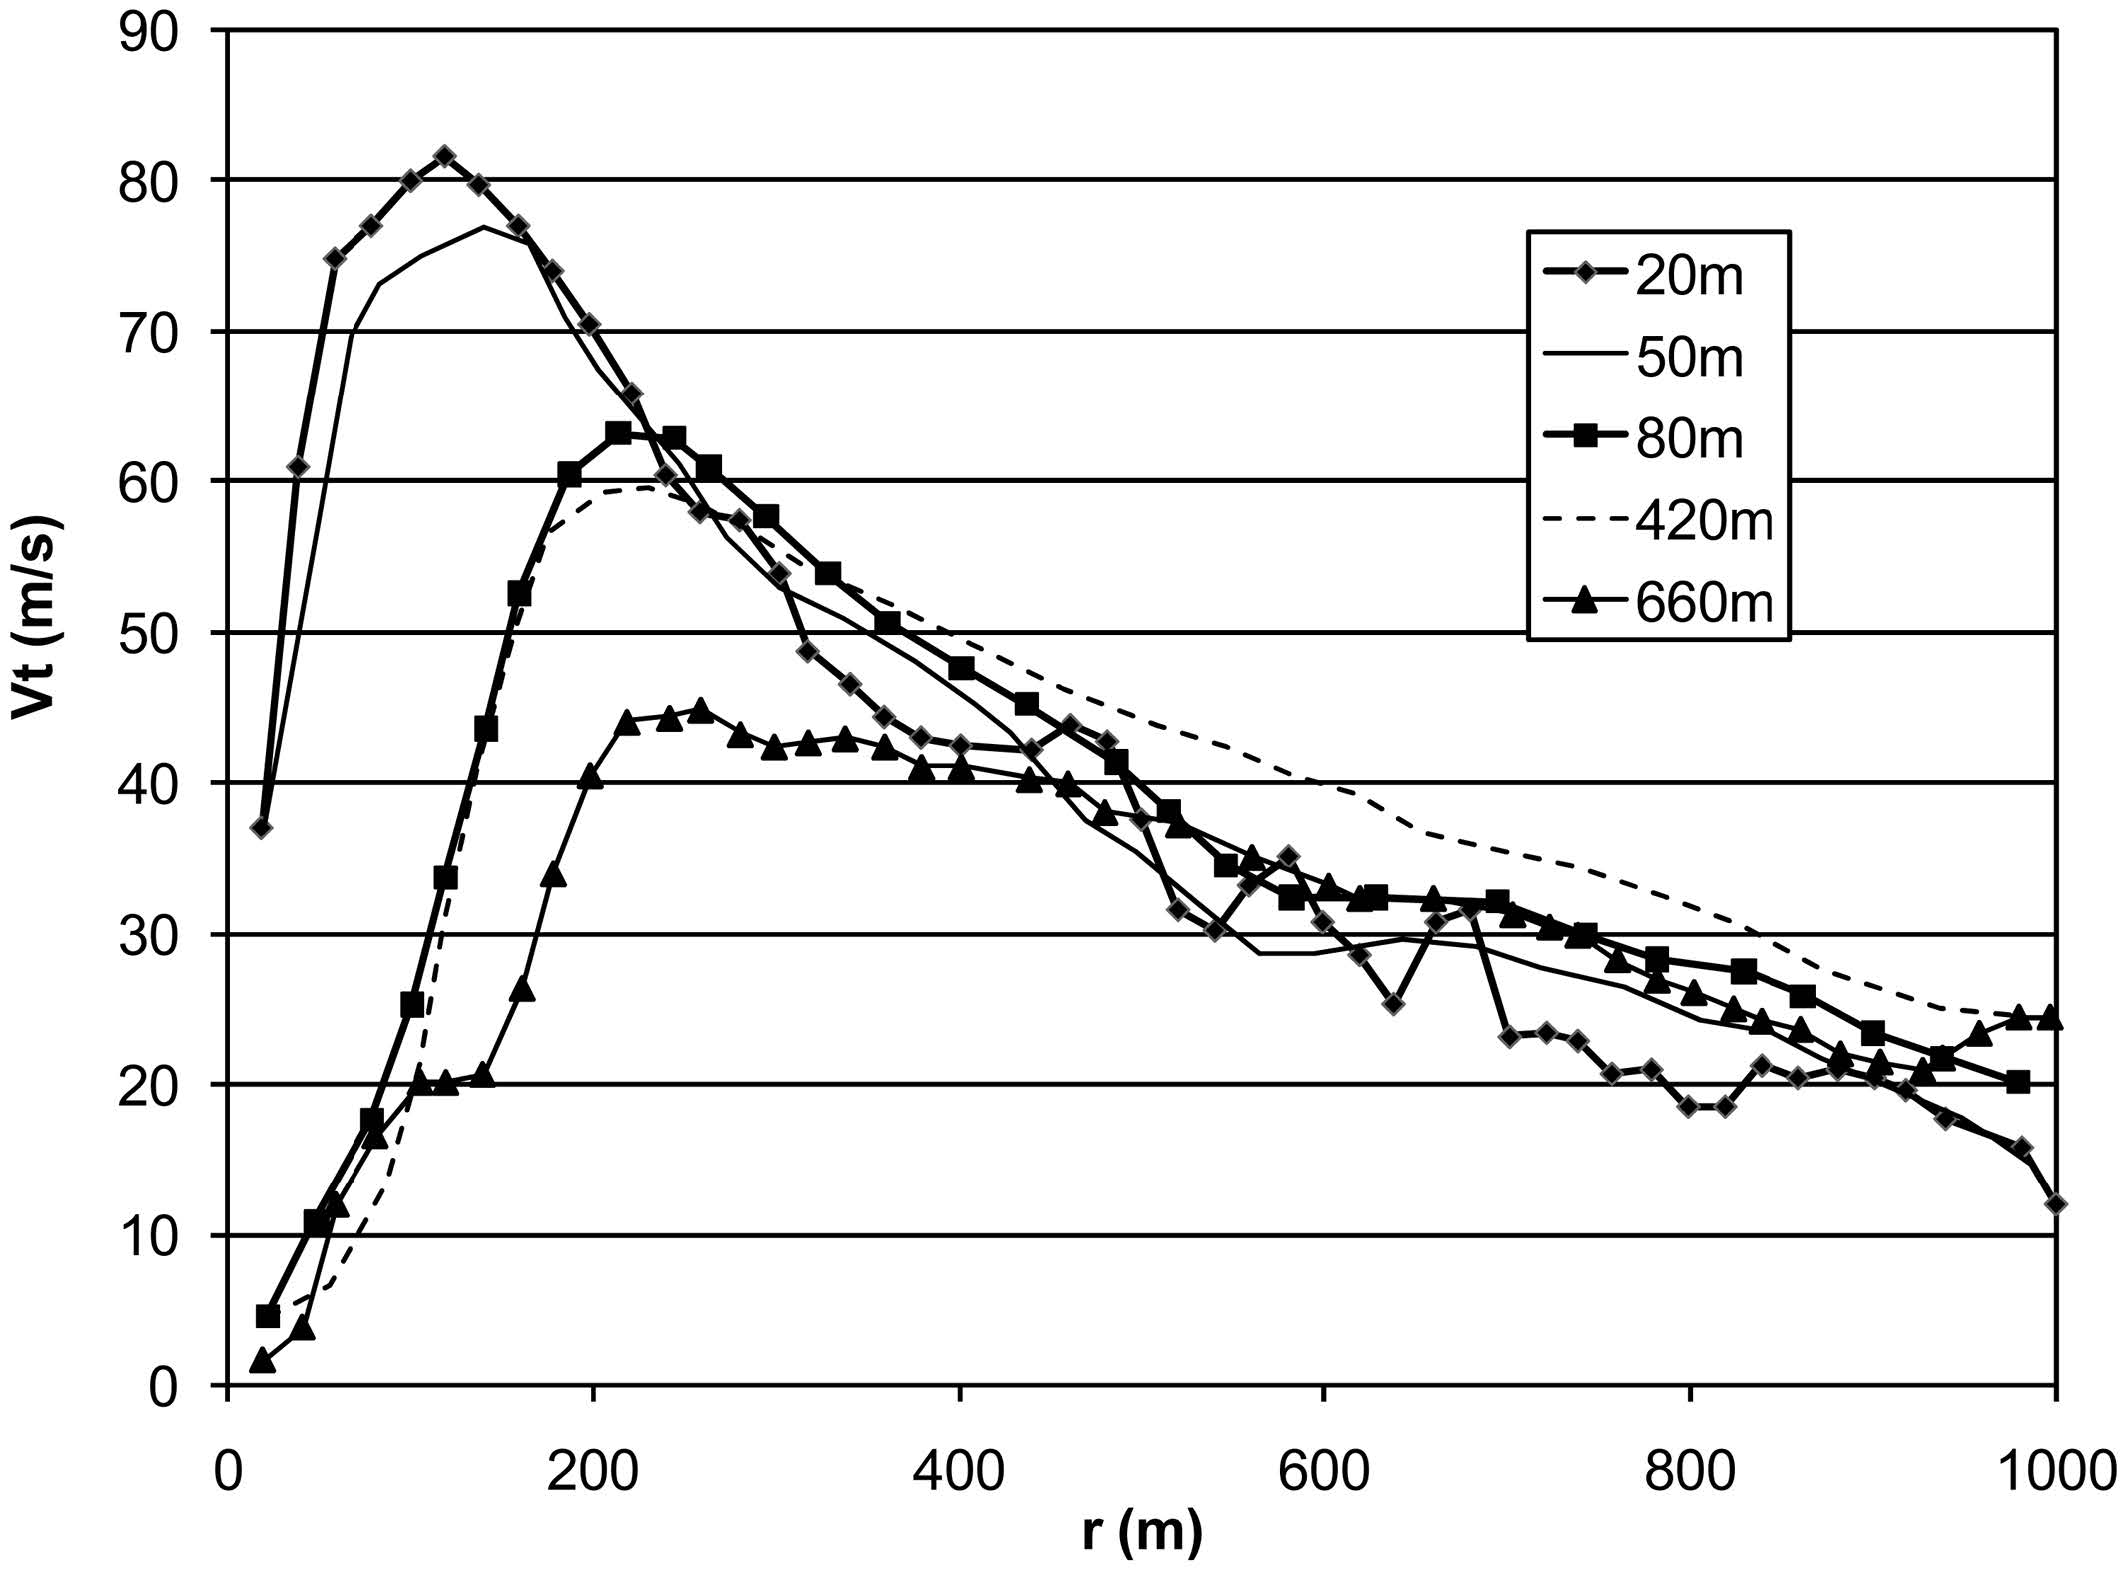
\includegraphics[width=0.6\textwidth]{spencer-vt.jpg}
    \caption{龙卷风切向风速沿径向的分布曲线}
    \label{fig:vt}
\end{figure}

\begin{figure}[!htbp]
    \centering
    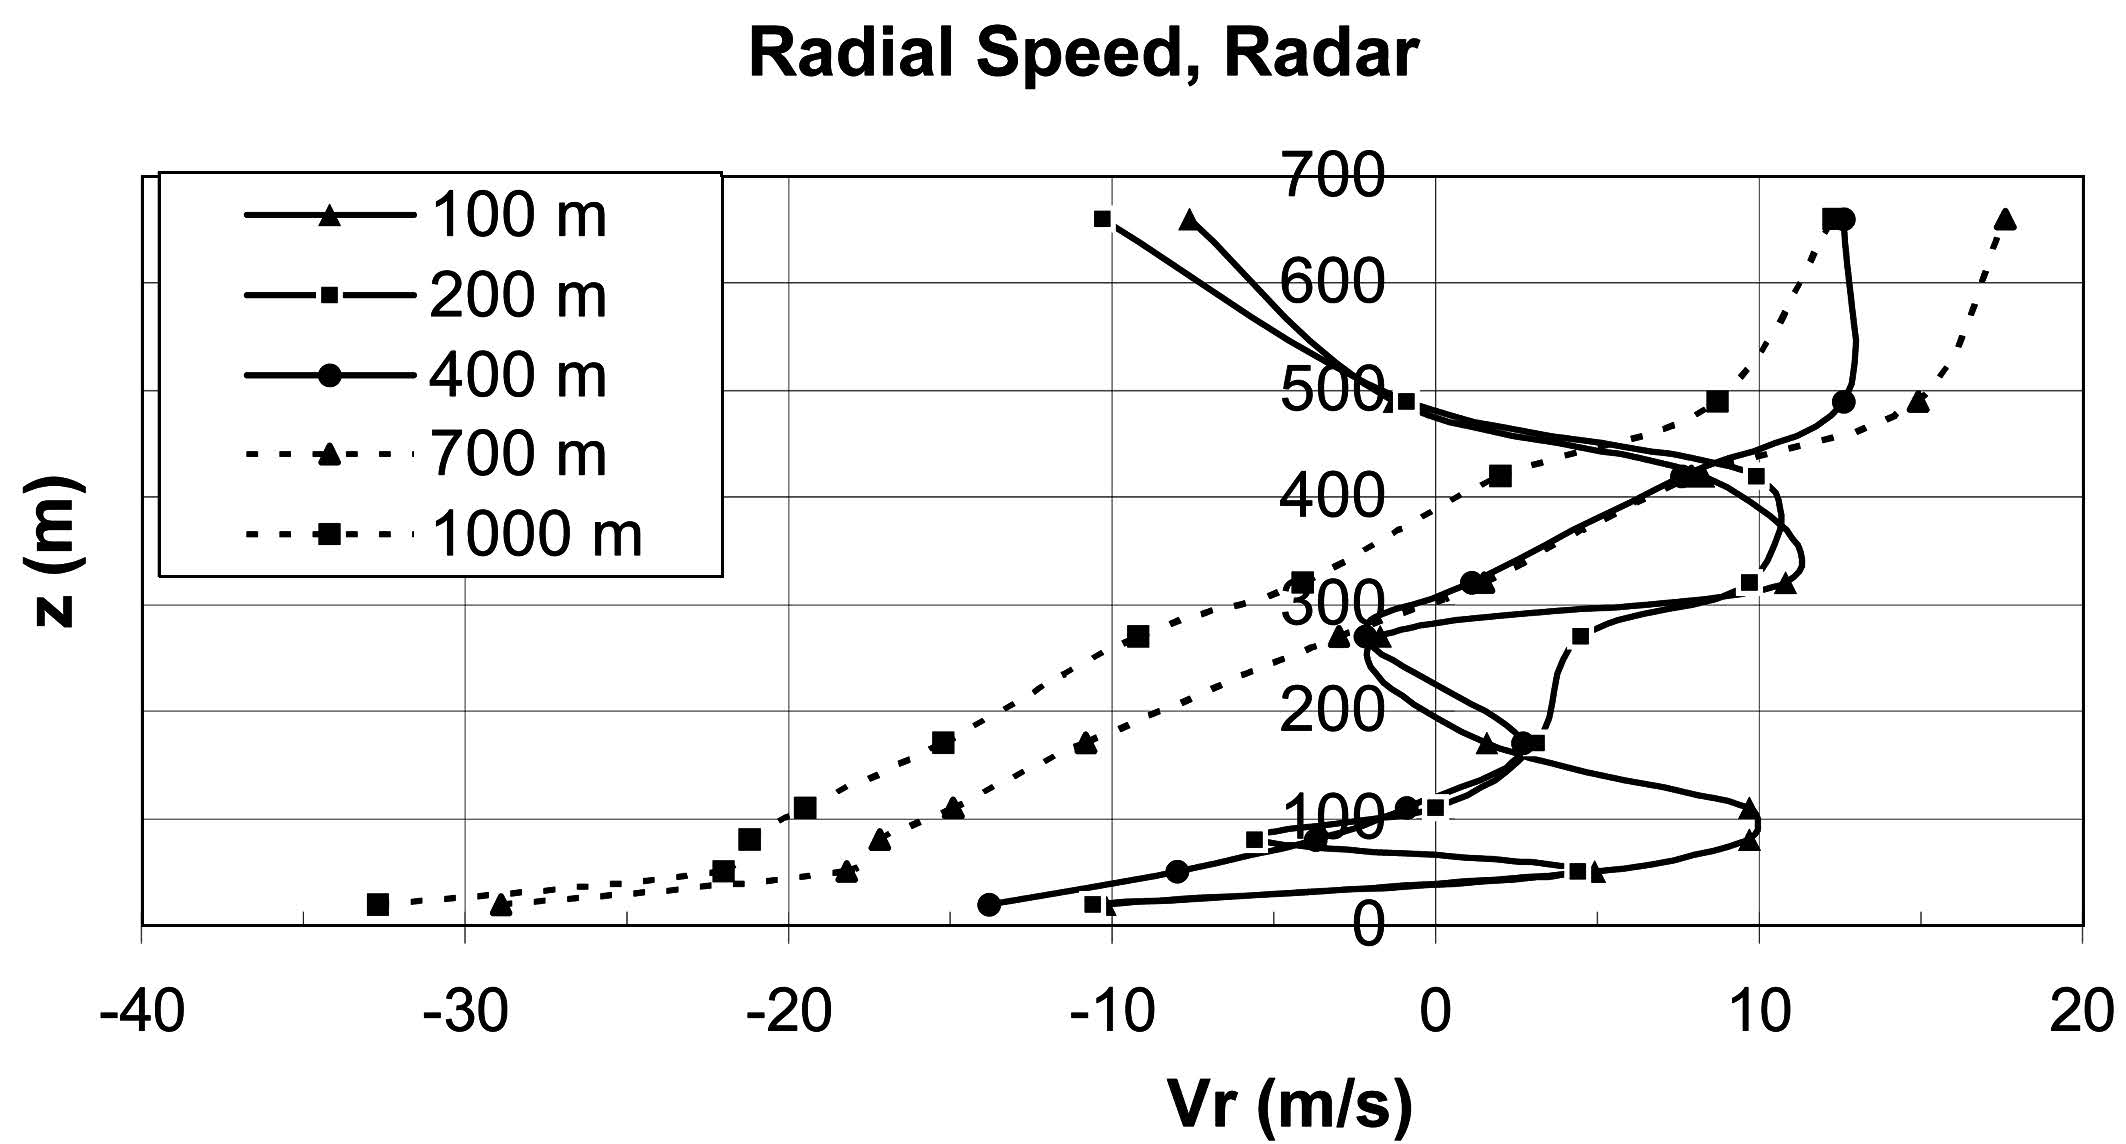
\includegraphics[width=0.6\textwidth]{spencer-vr.jpg}
    \caption{龙卷风径向速度沿高度的分布曲线}
    \label{fig:vr}
\end{figure}

图\ref{fig:vt}为所测得的 \SI{20}{m} 到 \SI{660}{m} 高度处龙卷风的切向风速曲线。
龙卷风的切向风速曲线存在一个峰值,其核心半径随高度从\SI{120}{m}变化到\SI{250}{m},表现为漏斗形状。
图\ref{fig:vr}为龙卷风在不同径向位置处,径向风速随高度的变化曲线。
负值表示空气流入龙卷风内部,在离龙卷风中心\SI{1000}{m}处,\SI{400}{m}以下均为入流层。
但随着距离龙卷风中心距离越来越近,入流层的厚度逐渐减小。
最大径向速度出现在地面以上\SI{20}{m}高度处,这是雷达所能测得最低位置处的风速值。

目前龙卷风野外实测最大的研究项目是 VORTEX2 实验。
它是由美国科学基金会(NSF)和美国海洋和大气局(NOAA)共同组建,耗资 10 亿美元,
共有 100 多位研究者参与其中,出动雷达车共 10 部,启用近 40 个移动地面气象站,风暴边缘利用直升飞机探测。
该项研究的现场实测部分从 2009 年 5 月 1 日开始,于 2010 年 6 月 15 日结束。
所观测的范围从美国德克萨斯州的西部直到明尼苏达州的西南部,长达 1448 公里。

该项研究主要为了解决以下几个简单却很难回答的基本问题:
龙卷风是什么时候怎样形成的,为什么有些强烈并持续时间长而有些微弱且持续时间短;
龙卷风的结构是怎样的,它们靠近地面的风速有多大,是怎样对周围造成破坏的;
怎样可以更好地预报龙卷风,目前能提前预报龙卷风的时间平均为 13 分钟,
并且有 $70\%$的错误率,怎样可以更准确地预报,并且增加提前预报的时间。
初步数据显示 VORTEX2 一共捕获大约 30 个较大级别的龙卷风,
20 个强度较弱或寿命较短的龙卷风,其中有些龙卷风超过了 EF2 级。
所采集的龙卷风数据已在整理分析当中,但所测龙卷风原始数据的讨论和发表工作要在现场实测完成后的 5至7年内才能完成。

\subsection{试验模拟研究}
由于现场实测的困难和限制,研究者尝试建立缩尺龙卷风发生装置模拟龙卷风风场及其对结构的作用。
Chang \cite{chang1971tornado}在 1971 年最早使用实验装置模拟龙卷风,得到了内部风场的切向速度和径向速度,
发现这可作为有限的现场实测的补充,是一种有效的方法。
1972 年 Ward \cite{ward1972exploration}改进了 Chang 的龙卷风模拟装置,
改进的装置能仅允许近地面空气进入,并设置了滤去气流竖向涡量的蜂窝板。
此后许多龙卷风发生装置均是基于这个装置的改进。
1977 年普渡大学的 Church \cite{church1977tornado}设计了新型龙卷风模拟装置,采用旋转金属网实现气流的旋转。
1993 年 Lund 和 Snow为普度大学第二代龙卷风模拟装置中使用了激光多普勒测速仪,发现模拟的龙卷风风场的竖向速度、径向速度和切向速度的分布符合 Rankine 涡的特征。
该装置还采用了导流板代替了旋转的金属网,可以产生不同角度的入流速度。
2008 年 Mishra \cite{mishra2008physical}利用新的龙卷风模拟装置模拟出了速度场,并与 1998 年 5 月 30 日发生的曼彻斯特龙卷风和 2003 年 7 月 24 日发生在南达科他州的实测数据进行了对比,
发现二者的压力分布和切向速度分布吻合较好,这表明利用实验模型模拟龙卷风是可行的。
2008 年 Haan \cite{haan2009tornado}研究了不同龙卷风模拟装置设置对龙卷风涡结构及其大小的影响。

由于龙卷风发生装置可有效模拟龙卷风风场结构,研究者开始将不同类型的建筑物放置在发生装置中,用来研究龙卷风荷载。
1983 年 Jischke \cite{jischke1983laboratory}利用类似于 Ward 型龙卷风研究了圆柱形和长方体建筑物在龙卷风风场表面的风压分布,发现其与常规风洞实验的结果相差甚远,即建筑物表面受到的风压是在常规风场中的 3 至 5 倍,并指出龙卷风的最大风速、建筑模型的位置以及建筑模型与涡的相对方位是龙卷风造成破坏的重要因素。
2003 年爱荷华州立大学设计建成了可平行移动的龙卷风发生装置,内部可放置缩尺比 $1/150$ 到 $1/300$ 的结构模型。
2006 年,爱荷华州立大学的 Sarkar 和 Haan \cite{haan2009tornado}对 \SI{54}{m}宽,\SI{216}{m}高的缩尺比例为$1/500$ 的长方体房屋进行了研究,发现当龙卷风等级为 F2 级时,龙卷风荷载超过了美国土木工程师协会(ASCE7-02)规定的荷载值,约为美国沿海地区风荷载的 1.8 倍。
2008 年 Mishra \cite{mishra2008physical}利用德州理工大学的漩涡 2 号模拟装置(TTU-VSII)对不同径向位置处立方体建筑上的龙卷风作用进行了实验研究,给出了可渗透建筑(其内部的压力与龙卷风压相平衡)的表面压力系数。
研究表明,当建筑物位于所模拟龙卷风的边缘时,只有一个面为正压,这与大气边界层流中的情况比较类似。
随着建筑物不断靠近龙卷风中心,龙卷风的涡流影响越来越大。
2010 年 Haan \cite{haan2009tornado}等人利用爱荷华州立大学(ISU)的移动龙卷风模拟装置模拟人字屋顶建筑上的龙卷风荷载。
实验结果表明,建筑侧面风吸力的峰值是吹直风时的 $1.5$ 倍,竖向力系数峰值是一般规定的 $2$ 到 $3$ 倍,这可能是由于龙卷风中心存在较大负压的影响。
2012 年 Sabareesh 等人\cite{sabareesh2012dependence}通过东京理工大学的龙卷风模拟装置,研究了固定龙卷风中不同位置及地形环境中的建筑物表面风压分布情况。
当建筑物位于龙卷风核心半径处时,与切向流相垂直建筑表面的负压相对于其他表面较小。
2013 年 Rajasekharan \cite{rajasekharan2013characteristics}利用东京理工大学的龙卷风模拟装置,研究了建筑物在龙卷风中的位置以及两种不同开洞方式对建筑物内部压力、屋顶净风力的影响。

国内龙卷风方面的试验研究起步较晚,2013 年,东南大学的汤卓等建造了国内首个龙卷风发生装置,并将其命名为“龙卷风塔”,该试验装置如图\ref{fig:seu-tornado}和图\ref{fig:seu-tornado2}所示。
\begin{figure}[!htbp]
    \centering
    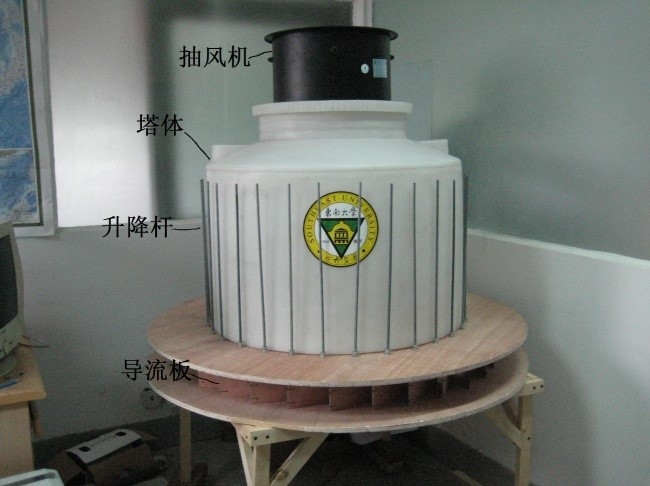
\includegraphics[width=0.6\textwidth]{tornado-sim.jpg}
    \caption{东南大学汤卓龙卷风发生装置}
    \label{fig:seu-tornado}
\end{figure}

\begin{figure}[!htbp]
    \centering
    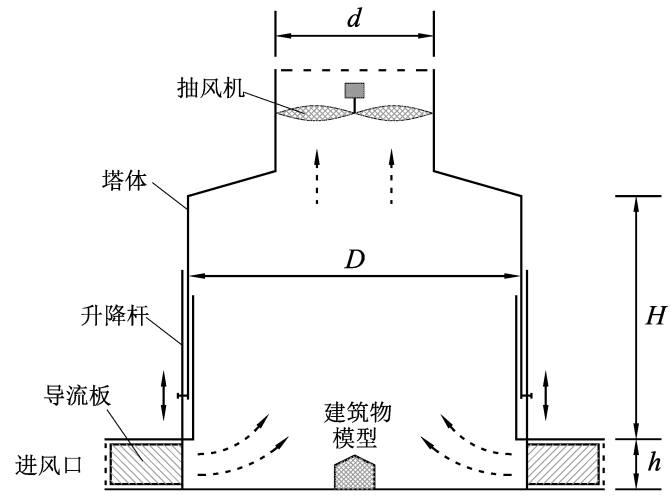
\includegraphics[width=0.6\textwidth]{tornado-sim2.png}
    \caption{东南大学汤卓龙卷风发生装置原理图}
    \label{fig:seu-tornado2}
\end{figure}

利用此装置进行了龙卷风作用下双坡屋面风压分布的试验研究,结果表明:
龙卷风场的风速分布、风压分布以及总气压降和 Rankine 涡模型吻合较好,其试验结果也说明了龙卷风作用于建筑物的荷载与常规风作用存在较大差异。
2014 年,同济大学的王锦和周强等\cite{wang2014tornado}制造出了龙卷风试验装置。
该试验装置是基于 Haan 等的设计原理制作而成的,主要由顶部悬吊的控制风机、环状管道以及导流板组成。
该装置可以产生一定的平移速度,最大为 \SI{0.4}{m/s},试验过程中采用眼镜蛇探头测试龙卷风风场。
试验结果表明其模拟的切向速度和静压分布与真实龙卷风的监测结果较一致。

\subsection{数值模拟研究}
龙卷风的现场实测具有许多限制,难以准确观测近地面处(\SI{20}{m} 以下)的真实风场,
这限制了现场实测数据在实际工程抗龙卷风设计中的应用,因为近地面风场是工程设计主要关注的;
再者,龙卷风的解析模型(如 Rankine 模型)是经过简化的理想模型,还不能贴近真实风场;
最后,即使是试验方法也受到缩尺比的限制,难以模拟真实龙卷风尺寸。
研究者开始寻找新的研究龙卷风的方法。

龙卷风数值模拟方法的研究,主要是在龙卷风缩尺试验研究的基础上发展起来的。
1997 年,Lewellen 等人\cite{lewellen1997large}利用大涡模拟技术(Large Eddy Simulation, LES)模拟了一个单涡龙卷风结构,
并研究其与地面的相互作用,解释了形成龙卷风结构所需的条件,
还指出 Rankine 涡模型是满足 Navier-Stokes 方程的最简单模型。
1999 年 Nolan 和 Farrel \cite{nolan1999structure}利用轴对称不可压缩流的数值模型研究了龙卷风结构的动力特性和结构特性,
发现旋转流场的角动量和湍流粘度直接影响龙卷风的结构。
2003 年 Selvam 和 Millett \cite{selvam2003computer}利用 Rankine 涡模型给出了数值模拟龙卷风风场的速度边界条件,
并利用 LES 方法计算了立方体表面作用的龙卷风荷载,
发现平移的龙卷风模型产生比准定常模型更大的作用力,墙体要增加$45\%$,屋顶要增加将近一倍。
2008 年 Kuai 等人\cite{kuai2008cfd}以爱荷华州立大学的龙卷风模拟装置为基础进行了数值模拟,
表明数值模拟结果可较好吻合实验数据,若考虑地面粗糙度,数值模型可更好模拟雷达观测的数据。
2011 年 Nashimi 等人\cite{alrasheedi2011computing}利用 LES 方法对同一龙卷风尺寸,不同建筑物尺寸(建筑平面尺寸从一倍变到八倍,高度保持不变),
龙卷风和平行常规风分别作用于建筑物的荷载进行了对比研究,
发现随着建筑物平面尺寸的增大,龙卷风风场中建筑物的竖向阻力系数最多可减少$80\%$,
侧向阻力系数和轴向阻力系数最多可减少$90\%$。
2012 年 Natarajan 等人\cite{natarajan2012large}利用 LES 方法研究龙卷风平移速度及地面粗糙度对龙卷风风场的影响,
发现随着地面粗糙度的增加,减小了模拟龙卷风的最大切向速度,
而龙卷风平移速度对风场最大切向速度的影响不能得到统一结论,切向速度出现减小和略微增大两种不同情况。

国内针对龙卷风的数值模拟研究日趋增多。
2005 年同济大学的陈艾荣\cite{chen2004large}基于准定常理论对大跨斜拉桥在龙卷风作用下的响应做了分析研究,发现了龙卷风对斜拉桥的竖向托起效应。
2009 年湖南大学的甘文举\cite{gan2009low}通过涡运动理论,建立了考虑龙卷风平移运动的数值风场模型,对低层房屋的龙卷风荷载及抗风设计提出了实用计算的建议。
2011 年,河北大学刘伟\cite{liu2011lou}采用了 Realizable 湍流模型模拟了龙卷风风场特性,并模拟了不同体型的建筑物位于风场中不同位置时的受力情况。
同年,哈尔滨工业大学李波利用 Fluent 对影响龙卷风风场的各种参数进行了分析,还得到了风场中建筑物表面和附近的速度与风压的分布特征。
2012 年,东南大学汤卓\cite{tang2012tornado}利用 CFD 数值模拟方法模拟了龙卷风作用于大跨穹顶结构的研究,获得了大跨穹顶结构表面的风压系数和作用在结构上的龙卷风荷载时程曲线,并对大跨穹顶结构作了风致响应分析。
2012 年,哈尔滨工业大学徐枫\cite{xu2013tornado}采用 Fluent 模拟了龙卷风风场特性,并对比理论模型从而验证了模拟结果的合理性。
2013 年,唐飞燕\cite{tang2013tornado}探讨了龙卷风风场中沙粒对结构冲击作用。
2014 年,东南大学王兆勇\cite{wang2015different}利用湍流模型模拟了在等效移动龙卷风作用下不同坡角的双坡屋面模型的风压分布特征,并与静态龙卷风风场特性相比,发现等效移动龙卷风风场中风压激增现象更加明显,双坡屋面风荷载急剧增大。

\section{本课题研究现状}
目前国外研究龙卷风作用下输电塔结构响应的文献较少。
Savory(2001)\cite{savory2001modelling}采用龙卷风 Wen 模型(忽略龙卷风风场竖向速度),利用风力系数将风速场转化为输电塔结构所受的风荷载,并考虑了龙卷风的平移运动,在其行进路径垂直于输电线的典型工况下进行动力时程分析,并根据输电塔结构的动态响应分析其破坏形态。
Langlois(2007)\cite{langlois2007design}主要评估了 ASCE、Behncke 等提出的多种龙卷风简化荷载模型对输电塔结构响应的影响。
其中的龙卷风简化荷载模型假定输电塔所受的风压是均匀分布的,并且忽略了风场的竖向分量及风场对输电线的作用。
Hamada(2010)\cite{hamada2010finite}利用缩尺 CFD 模型进行龙卷风风场的数值模拟,然后根据 ASCE No.74 规范提出的计算方法将 CFD 风场转化为输电塔结构受到的风荷载,然后进行静力弹塑性分析。
并改变龙卷风核心相对于输电塔结构的位置,分析其对输电塔结构响应的影响。
Hamada(2011)还进行了考虑龙卷风平移运动时输电塔结构动力时程分析,思路与 Savory 类似,只是将龙卷风场采用 CFD 模拟风场,进一步考虑了龙卷风平移路径与输电线平行的工况。
Altalmas(2014)\cite{altalmas2014finite}研究思路与 Hamada 类似,进行了更详尽的参数分析,即龙卷风核心相应于输电塔的角度、距离这两个参数对输电塔结构响应最值的影响。

任超(2010)\cite{ren2010tower}仅考虑了龙卷风的平移速度和最大切向速度,利用《架空送电线路杆塔结构设计技术规定》的风荷载计算公式将其转化为输电塔结构受到的龙卷风荷载,进行静力弹塑性分析。
白俊峰(2011)\cite{bai2011tornado}利用 Rankine 龙卷风涡模型计算出空间桁架表面对应的风压,进行龙卷风作用下输电塔结构的静力计算,发现与相同风速下自然风作用下的结构响应很相近。

由此可见国内外文献研究龙卷风作用下输电塔结构响应的基本思路为:采用 Rankine 或 Wen 模型模拟龙卷风解析风场,或采用 CFD 技术模拟龙卷风数值风场;
然后利用规范中风荷载计算公式将风速场转化为风荷载并施加到输电塔有限元模型上,计算结构响应。
这一研究思路采用自然风作用下的风荷载参数(如体型系数等)计算龙卷风荷载,但龙卷风与自然风风场结构相差较大,有必要研究直接模拟输电塔结构所受龙卷风荷载的方法。
另一方面,国外的研究成果难以直接用于国内的输电塔结构抗龙卷风设计的参考,主要原因在于国内外输电塔结构体系存在不同之处,所以需要选取中国典型的输电塔工程进行建模计算;
另一个原因在于国内外将风场转化为风荷载的计算公式不同,因此需要利用中国规范或标准的风荷载计算公式评估龙卷风的作用。


\section{本课题主要研究内容}

输电塔结构是空间格构式塔架,其风荷载计算的传统方法主要依赖于风载体型系数。
然而,目前各国规范对格构式塔架的风载体型系数的取值有较大的差异;
另外对于格构式塔架这种特殊的结构形式,像多点测压这种对高层建筑、大屋盖结构风荷载测试十分有效的风洞试验方法却不适用。

故本文采用单向流固耦合方法计算龙卷风作用于输电塔结构的风荷载。
即在计算流体力学程序Fluent中直接建立输电塔的刚性模型作为流场计算的壁面,
再将CFD计算得到的壁面压力转化为结构有限元计算需要的风荷载。
这一方法不需依赖规范中风载体型系数,比风洞试验更为经济,
但具有如下难点:

\begin{itemize}
  \item 包含格构式塔架刚性模型的流域网格划分较为复杂。
  \item CFD计算得到的壁面风压数据量较大,如何转化为结构有限元计算的荷载?
  \item 如何在Fluent中模拟足尺龙卷风风场?
\end{itemize}

为解决流场网格划分复杂的难点,本文仅将输电塔主体框架在CFD计算流域中建模。
主要因为次要构件(如支撑等)截面尺寸较小,故本文忽略了其挡风效应,采用体型系数法计算风荷载。
这样做可大大减少流场网格数量,也降低了划分出质量较高网格的难度,CFD计算时间也能控制在可接受的程度。

为了将CFD计算得到的风压施加到结构有限元模型上,若采用壳单元可较容易实现CFD网格与FEA单元的映射,但结构采用壳单元模拟需要单元数量巨大,也要引入接触单元,这样有限元计算过于复杂。
故本文采用梁单元模拟输电塔结构,这就需要将CFD计算得到的风压数据转化为梁单元的节点集中力。
本文编制了这样的荷载转化程序,并设计了算例加以验证。

龙卷风数值风场的模拟已有大量的研究,本文在前人研究的基础上,选用Baker做的缩尺试验为基础建立了龙卷风缩尺风场,并与试验数据对比验证。
然后将龙卷风缩尺数值风场和1998年发生在Spencer地区的龙卷风实测风场进行对比,以引入长度相似比和速度相似比,并利用这两个相似比将缩尺风场改造成足尺风场(利用长度相似比将缩尺风场的计算流域放大,利用速度相似比将缩尺风场的入口风速放大)。


实现了利用单向流固耦合方法计算输电塔结构受到的龙卷风荷载后,本文还利用规范方法进行计算,从而可进行两种方法的对比。
选择龙卷风核心与输电塔中心的距离为龙卷风核心半径、袭击角分别为0度、45度和90度的典型工况,分别利用单向流固耦合方法和规范方法计算龙卷风荷载,进行龙卷风作用下输电塔结构的准静态分析,比较两种方法计算得到的结构代表性响应。


本文还进行了考虑平移运动的龙卷风作用下输电塔结构的动态响应分析。
由于采用CFD方法考虑龙卷风移动的计算量巨大,技术难度高,故本文采用规范方法计算龙卷风荷载。
首先根据龙卷风的平移运动,建立动态龙卷风风场及荷载模型。
并针对龙卷风运动典型工况(移动路径平行于输电线、移动路径垂直于输电线),分析输电塔典型节点所受龙卷风风速及风载时程,进行动力时程分析,提取结构位移响应时程曲线。

% 第二章:
% 建立龙卷风数值风场模型。
% 以 Baker 实验为基础,利用 Fluent 软件建立缩尺龙卷风风场模型,将 CFD 计算得到的数值龙卷风风场的风速分布与 Baker 实验进行对比,以验证模拟结果的正确性。
% 并将缩尺风场与实测 Spencer 龙卷风风场进行对比,引入足尺风场与缩尺风场的长度相似比和速度相似比,以探讨将缩尺龙卷风数值风场转化为足尺风场的方法。

% 第三章:
% 龙卷风作用下输电塔结构的静态响应分析。
% 利用单向流固耦合方法(下文简称 FSI)直接在足尺龙卷风风场中建立输电塔的刚性模型,进行 CFD 计算得到结构表面受到的龙卷风风压。
% 结构有限元计算采用梁单元模拟输电塔结构,故需研究将 CFD 计算得到的结构表面风压转化为梁单元节点集中力的方法。
% 本章还介绍了利用规范方法计算龙卷风荷载并施加到输电塔结构的方法。
% 最后改变龙卷风的袭击角度,分别在 0 度、45 度和 90 度工况下进行龙卷风荷载的计算和施加,
% 进行静态响应计算,并比较两种方法计算得到的结构轴向力和位移响应。

% 第四章:
% 龙卷风作用下输电结构的动态响应分析。
% 考虑龙卷风的平移运动,建立动态龙卷风风场及荷载模型。
% 针对龙卷风运动典型工况(移动路径平行于输电线、移动路径垂直于输电线),分析输电塔典型节点所受龙卷风风速及风载时程,进行动力时程分析,提取结构位移响应时程曲线。

%%% Local Variables:
%%% mode: latex
%%% TeX-PDF-mode: t
%%% TeX-engine: xetex
%%% TeX-master: "../main"
%%% End:
